\documentclass[11pt, letterpaper]{article}

\usepackage[pdftex]{graphicx}
\usepackage{amsbsy,amssymb,latexsym,amsmath}
 \usepackage{cite}
\usepackage{wrapfig}
\usepackage{algorithmic}
\usepackage{algorithm}
\usepackage{setspace}
\usepackage{epstopdf}
\usepackage{graphics}
\usepackage{subfigure}
\usepackage{setspace}
%\singlespacing
\onehalfspacing
%\doublespacing
%\setstretch{1.1}
%\usepackage{subfigure}


\include{definitions}
\def\tr{^{\,T}}
\def\*tr{^{\,*T}}
\def\inv{^{-1}}

\usepackage[left=1.1in,right=1.1in,top=1in,bottom=1in,letterpaper]{geometry}

\title{Disaggregation of Household Energy Consumption into Individual Appliances }
\date{\today}
\author{Kyung Woo Min, Muryong Kim, Min Lwin\\EE381V Project Report \\The University of Texas at Austin}

\begin{document}
\maketitle

\section{Abstract}
Even with advances in smart grid technology and a growing demand for cost-effective  energy consumption, detailed information about energy usage is often not available for residential electricity consumers. One reason is that energy usage is typically monitored at single point by the utility, only providing information on the aggregate power consumption.  In this paper, we attempt to disaggregate the energy usage data into specific appliances from single-point sensing measurements.  Our method involves extracting events from the time-series data to obtain relevant features.  We focus on two feature sets: low frequency and high frequency.  For each set, we create an event detection algorithm for feature extraction.  We present the results of our approach on a publicly available dataset.

\section{Introduction}

In this section, we provide the motivation and a brief description of the project.  A short discussion of related work in this area, including the methodology of previous competition winners is also provided.  This is followed by an overview of our approach, description of the raw data, and evaluation method.

\subsection{Project Description}

This project follows the Belkin Energy Disaggregation Competition on kaggle.com \cite{Kaggle}. The goal is to disaggregate household energy consumption into individual appliances. Appliances with switched mode power supplies (SMPS) generate electromagnetic interference (EMI) due to the high frequency switching and will generate noise in the voltage waveform near their switching frequency. Therefore, each type of appliance will have its own frequency-domain signature, typically in the tens to hundreds of KHz. The dataset used for this project is publicly available on the competition website and contains voltage and current harmonics data for four households.  The dataset also contains high frequency noise (EMI) data for each household.  

Although the presence or absence of such EMI signatures and changes in voltage or current can indicate when a particular appliance is in use, classification can become challenging if the number of appliances in the home is large. Additionally, the signature of some appliances may drift or vary over time due to operating conditions and the mode in which they are used.  Predictive modeling is then required to make an inference about the appliance class given a particular signature.  The challenge is to accurately classify end-uses of energy at a fine-grained, appliance level. One application of this project is to continuously monitor real-time power consumption, broken down by electrical appliance.  Consumers can then view their energy usage and cost at a detailed enough level to determine cost-effective energy saving changes to usage patterns.  Based on the description above, our problem statement can be summarized as follows:

\begin{quote}
Using the harmonic and EMI measurements as features, the objective of this project is to build a multi-class classification model to determine which appliances are active at any given time (i.e, classify the active appliances based on harmonic and EMI signatures). 
\end{quote}



\subsection{Summary of Related Work}

From our literature survey, several relevant papers were found in the area of energy disaggregation \cite{EMI,emisurvey,mit,adaptive,prob}.  In the following section, we have provided a brief summary of the two most relevant papers to this project.  Each presents an approach to solve the same problem, however, using different feature sets: low frequency aggregate power consumption and high frequency voltage EMI. Additionally, the methodology of the competition winners is provided.

\subsubsection{Literature Survey Summary}

Prior research in this area has focused on the use of aggregate power consumption patterns as features to identify what appliance is being used and how much energy it is consuming. In particular, the authors in \cite{mit} discuss various approaches in nonintrusive load monitoring.  These include detecting changes in steady-state power measurements and characterizing them as differnt events.  Only the real and reactive power of the fundamental frequency is observed, creating a two-dimensional feature space.  Some challenges reported by the authors include different loads not exhibiting unique signatures in the 2D features space and the difficulty in determining steady-state features due to turn-on transient noise.  Some recommended advanced techniques are to include the 3rd order harmonics as a feature and using turn-on transients for event detection.  

An alternative approach is to examine the EMI signatures of electronic appliances as identifying features \cite{EMI}. The authors attempt to classify the transient noise that is generated by the high frequency switching of devices in a household. The paper utilizes a novel feature extraction method by modeling the EMI noise signature with a Gaussian function with its mean at the switching frequency.  The paper shows that their method is robust to simultaneous devices and can detect overlapping device activation events.    

For detected events, a Gaussian curve is fit to the high frequency signature with features for the center, width, and amplitude of each peak.  These three parameters become the extracted features to be used in the K-Nearest Neighbor classifier, with K=1 and a Euclidean distance metric with inverse weighting. Some difficulties encountered by the authors are: multiple similar devices, light dimmers, simultaneous events, end user calibration and phase coupling. One example of such issues is how the switching frequency of some TVs change depending on the screen brightness.  Therefore, the high frequency signature will shift depending on what is displayed on the screen.  The event detection algorithm will report each of these new peaks as new events.  

\subsubsection{Approach of Competition Winners}
A detailed description of the methods used by the competition winners is not provided on the website. However, some of the successful participants posted their methodology in the competition forum \cite{Kaggle}.  Table \ref{winners} summarizes the methods used by the top three participants of the competition. One of the common characteristics of these participants was the use of a time difference to detect edges. However, insight into the data mining tools used by the top participants was not readily accessible.

\begin{table}[H]
\caption{Approach of Competition Winners}\label{winners}
\begin{center}
\begin{tabular}{|p{4.2cm}|p{11cm}|}\hline
\textbf{Participant} & \textbf{Approach}\\
\hline
J. Bombaz (Rank: 1st) & Used time differences to detect peaks.  Used the mean of two time windows to avoid the effect of noise.  Computed the similarity for applicances with unique characteristics. \\
\hline
L. Tandalla (Rank: 2nd) & Did not use the HF (high frequency) information.  Built a turning-on window and a turning-off window.  The windows runs through the time step to classify the test data.\\
\hline
N. Tene (Rank: 3rd) & Used time differences and edge detection algorithm to detect events.  \\
\hline
\end{tabular}
\end{center}
\end{table}


\subsection{Approach}

Our approach aims to combine the methods developed in \cite{EMI} and \cite{mit}. It focuses on both the low frequency aggregate power consumption data and high frequency voltage EMI data in order to utilize the classification strengths in each feature set.  In order to implement our approach we first need to convert the time series data to turn-on and turn-off events.  Therefore, accurate event detection is one of the primary focuses of our approach.  The advantage is a significant reduction in the size of data.  A drawback is that a reasonably accurate event detection method is required in order to minimize misclassification. The bulk of our effort in this project was spent in effective data pre-processing. A detailed discussion of the feature extraction methods will be presented in Chapters \ref{preprocess}, \ref{lfapproach}, and \ref{hfapproach}.  A brief summary of our classification methods is presented in Table \ref{classifiers}, which are discussed further in Sections \ref{lfapproach},  \ref{hfapproach}, and \ref{combined}. 

\begin{table}[h]
\caption{Classification methods}\label{classifiers}
\begin{center}
\begin{tabular}{|p{4.2cm}|p{11cm}|}\hline
\textbf{Classifier} & \textbf{Characteristics}\\
\hline
K-Nearest Neighbors & Classification using K-closest samples from the training set. \\
\hline
Decision Tree & Constructs multiple decision tree to reduce variability of using a single decision tree.	\\
\hline
Multi-Classifier Combining & Different appliances may be more suited to classification from only LF or HF data.  Combine output of different classifiers.\\
\hline

\end{tabular}
\end{center}
\end{table}


\subsection{Raw Data}
The project will utilize the complete dataset available from kaggle.com, provided by Belkin Energy. The set contains data from 4 homes (labeled H1-H4) consisting of both training and testing datasets. The training datasets are used to learn how each appliance in each home looks in terms of the EMI and harmonic signatures and build a model which can be applied to the test datasets for making predictions.  

For each home, the datasets include the first 5 harmonics of voltage and current measurements the FFT of the high frequency noise (captured every 1.0667 seconds).  The sampling rate is $f_s$ = 2 Mhz, which results in an FFT resolution of $f_r$ = 244.14 Hz. The dataset for each home is composed of several files.  For example, the data for H4 contains two training datasets and four testing datasets. The size and description of the files associated with each training and testing dataset are detailed in the tables below.

\begin{table}[h]
\caption{Example of Data Files for Each Training and Testing Dataset}\label{files}
\begin{center}
%\vskip -5pt
\begin{tabular}{|l|l|l|}\hline
\textbf{File name} & \textbf{Description} & \textbf{Data Size}\\
\hline
HF & spectrogram of high frequency noise & 4096 $\times$ 81000\\
\hline

TimeTicksHF &  UNIX timestamps corresponding to the HF & 81000$\times$1\\
 \hline

LF1V & fundamental and first 5 harmonics of 60Hz voltage of Phase-1. & 517067$\times$6\\
 \hline

LF1I & fundamental and first 5 harmonics of 60Hz current of Phase-1. & 517067$\times$6\\
 \hline

TimeTicks1 & UNIX timestamps corresponding to Phase-1 current and voltage. & 517067$\times$1\\
 \hline

LF2V & fundamental and first 5 harmonics of 60Hz voltage of Phase-2. &  517066$\times$6\\
 \hline

LF2I & fundamental and first 5 harmonics of 60Hz current of Phase-2. & 517066$\times$6\\
 \hline

Timeticks2 & UNIX timestamps corresponding to Phase-2 current and voltage. &  517066$\times$1\\
 \hline

TaggingInfo & labels for training purposes (For Training Data only) & 35$\times$4 \\
\hline
\end{tabular}
\end{center}
\end{table}


\begin{table}[H]
\caption{Total Number of Classes and Datasets for Each Home}\label{classes}
\begin{center}
\begin{tabular}{|c|c|c|c|}
\hline 
\textbf{House No.} & \textbf{No. of Classes} &\textbf{ No. of Training Sets} &\textbf{ No. of Test Sets}\tabularnewline
\hline 
H1 & 38 & 6 & 4\tabularnewline
\hline 
H2 & 37 & 4 & 4\tabularnewline
\hline 
H3 & 37 & 3 & 4\tabularnewline
\hline 
H4 & 36 & 2 & 4\tabularnewline
\hline 
\end{tabular}

\end{center}
\end{table}

The observations recorded in each training and testing dataset cover approximately 24 hours.  Therefore, the files in Table \ref{files} for each training and testing dataset listed in Table \ref{classes} have approximately the same sizes.

\subsection{Evaluation}
Although the competition has completed, the accuracy of our model will be evaluated using the same method as in the competition, using mean Hamming Loss \cite{Kaggle}. The formulas are given by,
\begin{equation}
\text{HammingLoss}(x_i,y_i) = \frac{1}{|D|}\sum_{i=1}^{|D|}\frac{xor(x_i,y_i)}{|L|}
\end{equation}
where,\\
$|D|$ is the number of samples (timepoints)\\
$|L|$ is the number of labels (applicances)\\
$y_i$ is the ground truth\\
$x_i$ is the prediction.\\
\begin{equation}
\frac{1}{|H|}\sum_{j=1}^{|H|}{\text{HammingLoss}_j}
\end{equation}
where,\\
$|H|$ is the number of homes. Additionally, the performance of our model will be compared with the posted scores of the top participants as listed on the website.  The competition requires submittal of solutions on a standardized .csv file.  Depending on the home, the submittal file specifies between 1001 to 1880 unique timestamps from the test data. For each specified timestamp, we must predict whether each appliances is on or off.  Therefore, the total number of predictions required for all test datasets is 219,579.      



\section{Data Pre-Processing}\label{preprocess}

This section aims to provide a description and methodology of the major pre-processing steps taken.  This includes discussion of some of our initial feature extraction attempts that are not utilized in the final model.

\subsection{Applying Domain Knowledge}

Before proceeding with other data pre-processing techniques, we first apply our domain knowledge to the problem and extract relevant features.  The raw dataset contains measurements of voltage, current, and high frequency EMI.  When an appliance turns on, we expect negligible change in the fundamental voltage component, but a detectable change in the fundamental current component.  Because this is equivalent to a change in power consumption, the raw voltage and current data is used to calculate complex power, S, and is separated into real and imaginary components (S = P + jQ).  As in \cite{mit} we have transformed the raw data into a two-dimensional feature space of P and Q.

Although all appliances draw current when operating, it may not be a well separable feature as there may be overlap between several appliances. However, in the $\Delta$P and $\Delta$Q feature space, many devices are well separable as will be shown in later sections. Figure \ref{comparison} shows visualization of the training and testing data after converting voltage and current to the P and Q domain (red and blue curves denote different phases in the home).  Additionally, the raw EMI data is also shown for comparison.  It can be seen from this initial visualization that changes in P, Q, and high frequency EMI provide a promising feature set.


\begin{figure}[h]
\centering
\includegraphics[height=7.5cm]{fig/vis2.png}
\caption{Comparison of Training (left) and Testing Data (right)}\label{comparison}
\end{figure}


\subsection{Data Cleaning}
The dataset is provided by kaggle.com and does not require much data cleaning.  However, the following issues were encountered. In many instances of the training data, the ground truth labels for event turn-on or turn-off did not exactly match the power waveforms.  This can partially be observed in Figure \ref{comparison}, in the top left plot.  In some cases, the tagging label clearly misses the actual event.  Another type of error in the ground truth labels are events where turn-on and turn-off occur at the same timestamp.  Lastly, some events are observed in the P and Q data, but are untagged.  Due to these inconsistencies in the ground truth labels, a separate event detection algorithm is developed.

Another characteristic of this dataset is that training data is not representative of testing data.  In the training data, appliances are turned on and off, one at a time.  All appliances are then turned on and off approximately the same number of times.  However, in the testing data multiple appliances can be active at any time and the frequency of occurrence is not necessarily the same.  

\subsection{Data Reduction}

The size of the total dataset makes data reduction a key pre-processing step.  In particular, because we are dealing with high resolution time series data where appliances are turned on for only a fraction of the time, it is necessary to extract when appliances turn on or off and characterize these as events. Details on event detection is provided in sections \ref{lfapproach} and \ref{hfapproach}.

Additionally, the EMI data has high resolution in the frequency domain (4096 bins).  We tried two methods to reduce this data.  The first method was a Gaussian curve fit to difference vectors (see Figure \ref{gfit}), similar to the approach in \cite{EMI}. A sliding window average is used to smooth baseline noise. Then the difference between the sliding window average and the next FFT vector is used to find values that are greater than a predefined threshold, signifying an event. However, we deployed a multimodal Gaussian fit with three parameters for each mode: mean, scaling, and variance.  This provides a reduction from 4096 features to 9 features.  However, issues encountered with this approach are: deciding on the optimal number of modes for the entire data set for accurate event detection and the increased processing time to fit each function. 

\begin{figure}[H]
\centering
\includegraphics[height=4cm]{fig/gaussfit.png}
\caption{Example Gaussian Curve Fit to Difference Vector}\label{gfit}
\end{figure}



\section{Appliance Classification Using Power Consumption}\label{lfapproach}
This section concentrates on extracting the features in low frequency data.  In particular the voltage and current measurements at the fundamental frequency (50 or 60 Hz) are used to characterize the appliances given in the data.  Since every appliance consumes power when they are operating, the raw voltage and current measurements are preprocessed and the real power and the reactive power usages of each appliance are computed.  The procedures for calculating the real power and the reactive power include event detection, data smoothing, and power calculation.

\begin{figure}[h]
\centering
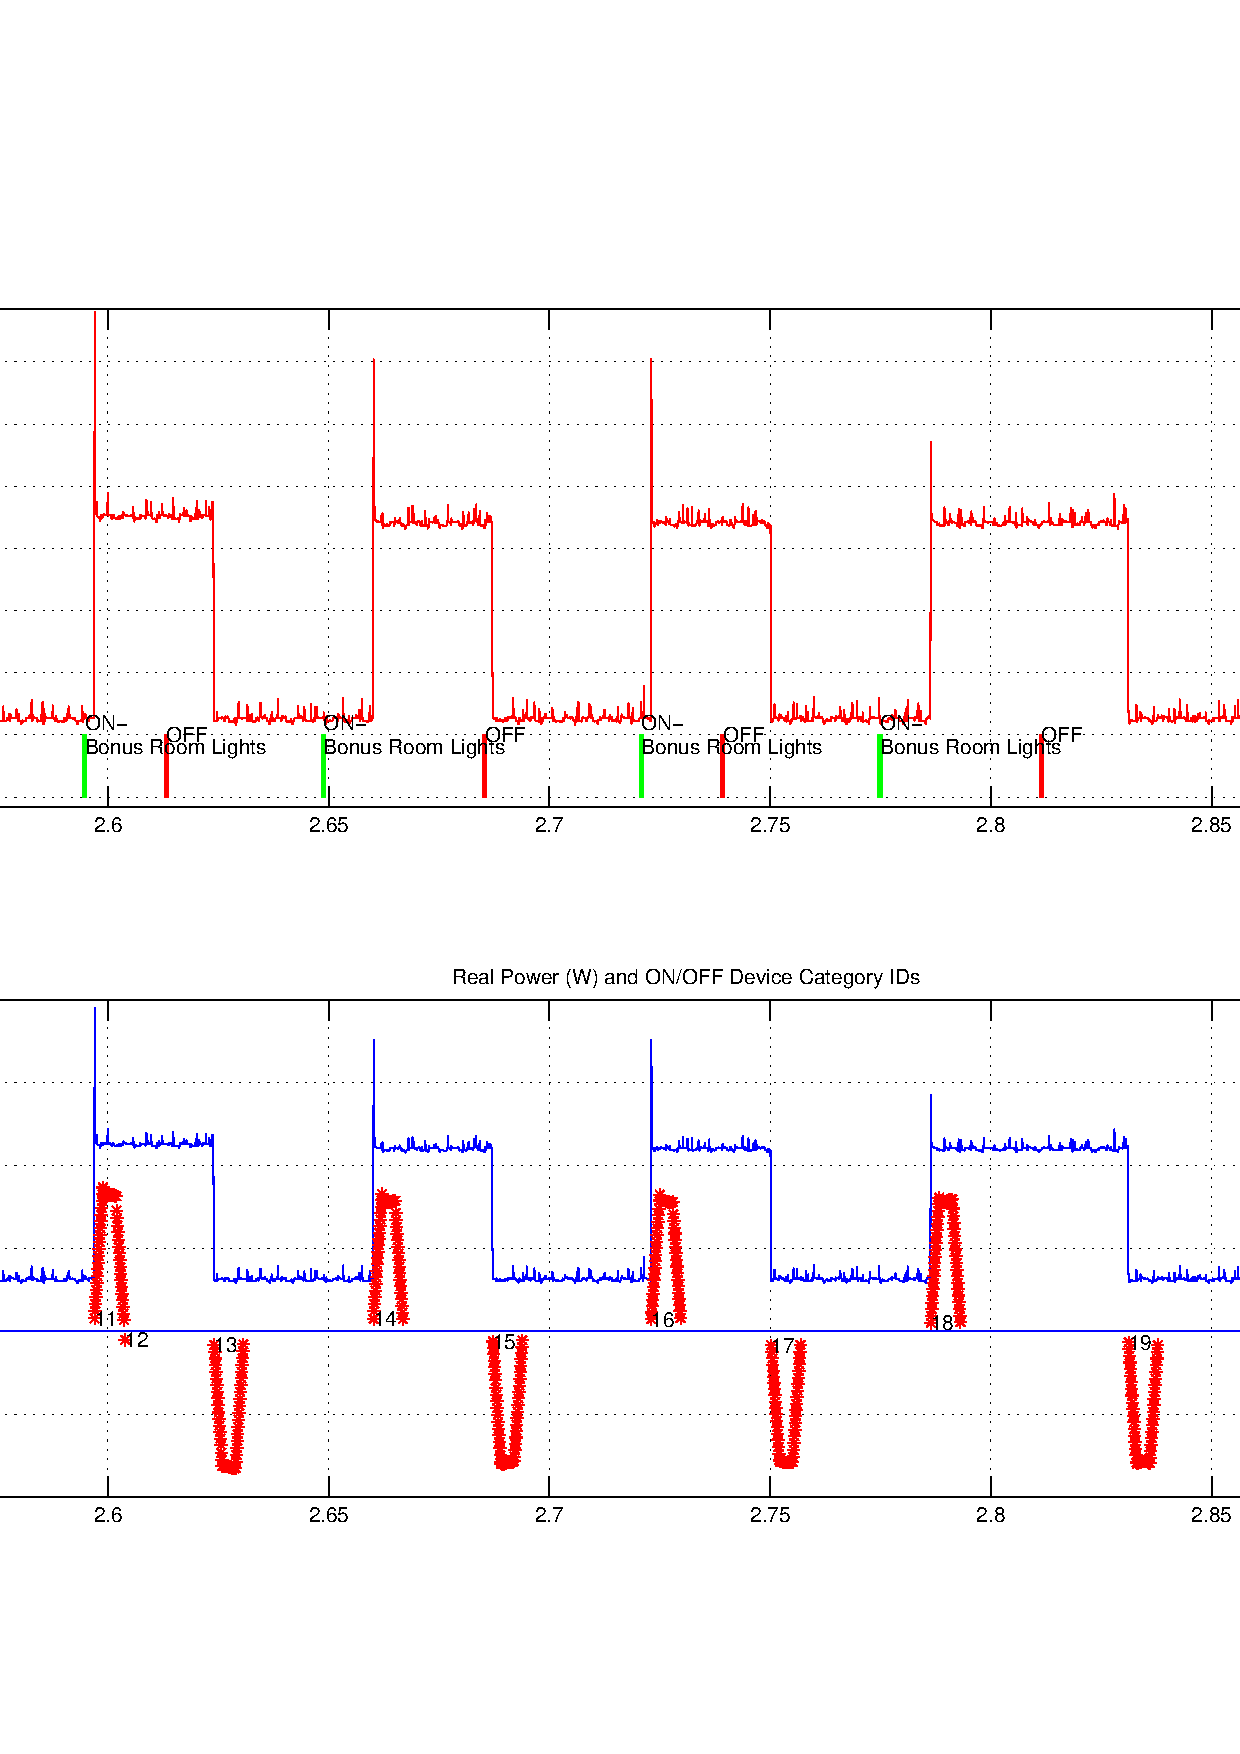
\includegraphics[height=4.5cm]{fig/rec.jpg}
\caption{A typical rectangular load shape}
\label{fig:rec}
\end{figure}

Note that when deriving the real and reactive power consumption, the load shape of each appliance is assumed to be rectangular.  Figure \ref{fig:rec} shows a typical rectangular load shape.  Many appliances turned out to have rectangular load shape and these appliances can be separated using real and reactive power consumption features.  Figure \ref{fig:PQ} shows feature space of appliances that have rectangular load shape.  The feature vector of each class are clustered together, implying that the real and reactive power features are sufficient for classifying most of the appliances.

\begin{figure}[h]
\centering  
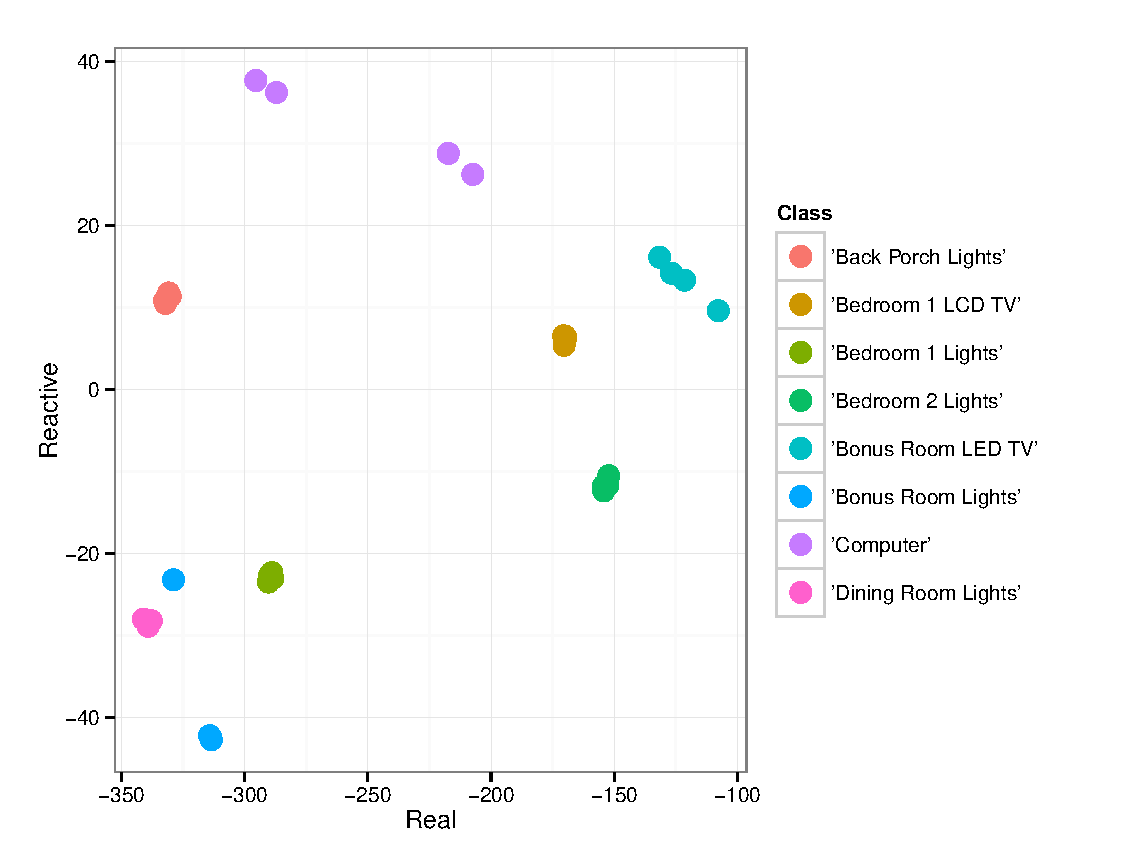
\includegraphics[height=6.5cm]{fig/ggplot.eps}
\caption{The appliances separated in real power and reactive power space}
\label{fig:PQ}
\end{figure}
 
\subsection{Event Detection Using Power Consumption Difference}
The exact time-index of the switching on/off time of the appliances should be detected in order to calculate the power consumption of each appliance.  The event detector is applied to both training and testing data for the following reasons.
\begin{enumerate}
\item{Training Data: the tagging info of the appliances is provided.  However, they do not represent the exact on and off time of the appliances.  In addition, there are multiple mislabels such as the on-label and the off-label indicating the same time index.  The event detector should be programmed separately to account for these offsets and mislabels.}
\item{Test Data: the tagging info is not provided.  The event detector should be able to capture when an appliance is switched on and off. }
\end{enumerate}

\begin{figure}[h]
\centering
\includegraphics[height=5.5cm]{fig/event.jpg}
\caption{Event detection using real power (left) and reactive power (right) differential waveforms}
\label{fig:event}
\end{figure}

The event detection in low frequency can be performed by using real power difference or reactive power difference.  However, the real power differences show better performance in the detection.  This is because most appliances are resistive and include internal power correction modules to maintain the unity power factor.  There are many cases when the reactive power does not change even if an event occurred.  From Figure \ref{fig:event}, the differences in the real power consumption are more notable than those shown for reactive power consumption. Therefore the real power differences is chosen to used as an event detector.  A threshold for the real power difference is set to indicate whether an event occurred.  If the threshold is too low, the event detector will indicate noise as an event and if is too high, some of the events might be neglected.

The differences in the real power consumption can provide additional information indicating whether the appliance is turning on or off.  Unless a power generator is included in the appliances list (not the case considered in the competition), positive power difference indicates that the appliance is turning on, and negative power difference indicates turning off.  

\subsection{Data Smoothing}
The purpose of data smoothing is to filter out the noise present in the real and reactive power waveforms so that actual power consumption of each appliance can be derived.
\subsubsection{Noise Reduction}
The power measurements have background noise coming from the measurement devices.  This noise will have an effect when deriving the actual power consumed at each appliance.  Assuming that the noise is Gaussian distributed, a moving average low-pass filter is applied to the entire data set to reduce the effect of the noise. Figure \ref{fig:lpf} shows the procedure in deriving the power consumptions after taking the low pass filter.
\begin{figure}[h]
\centering
\includegraphics[height=5.5cm]{fig/lpf.jpg}
\caption{N-tap moving average filter is applied to the power consumption waveforms}
\label{fig:lpf}
\end{figure}
\subsubsection{Impulse Noise Smoothing}
There are cases when a big impulse occurs at the incidence of switching on.  For training data, the effect of the impulse can be avoided by using the power differences in the falling edge. However, the impulses does effect the performance in the test data where the classification should be made in both switching-on and switching-off incidents.  Therefore, M-length windowed median filter is applied to the power consumptions data to filter out the impulses.
\begin{figure}[h]
\centering  
\includegraphics[height=5.5cm]{fig/med.jpg}
\caption{M-length windowed median filter is applied to the power consumption waveforms}
\label{fig:med}
\end{figure}

\begin{table}[h]
\caption{Parameter tuning}
\begin{center}
\begin{tabular}{|l|l|l|}\hline
\textbf{Tuning Parameter} & \textbf{Description}\\
\hline
Power difference threshold & Event detection\\
\hline
Window length of low-pass filter (N) & Reduces noise effect\\
\hline
Window length of median-filter (M) & Reduces impulse noise\\
\hline
\end{tabular}
\end{center}
\end{table}

\subsection{Phase Detection}
Most of the appliances are connected to the grid using single phase (phase 1 or phase 2) while some appliances which require higher voltage ratings are connected line-to-line (both phase-1 and phase-2).  Whether the appliance is connected to phase-1 or phase-2 is not used as an additional information.  This is because a house holder can connect an appliance at any electric plug and change the phase at any time.  However, line-to-line connected appliances will consume power from both phases regardless of their plugged-in location.  Figure \ref{fig:heater} illustrates this case.  ``Room basedboard heater" in Home 4 is consuming power from both phase-1 and phase-2.
\begin{figure}[h]
\centering  
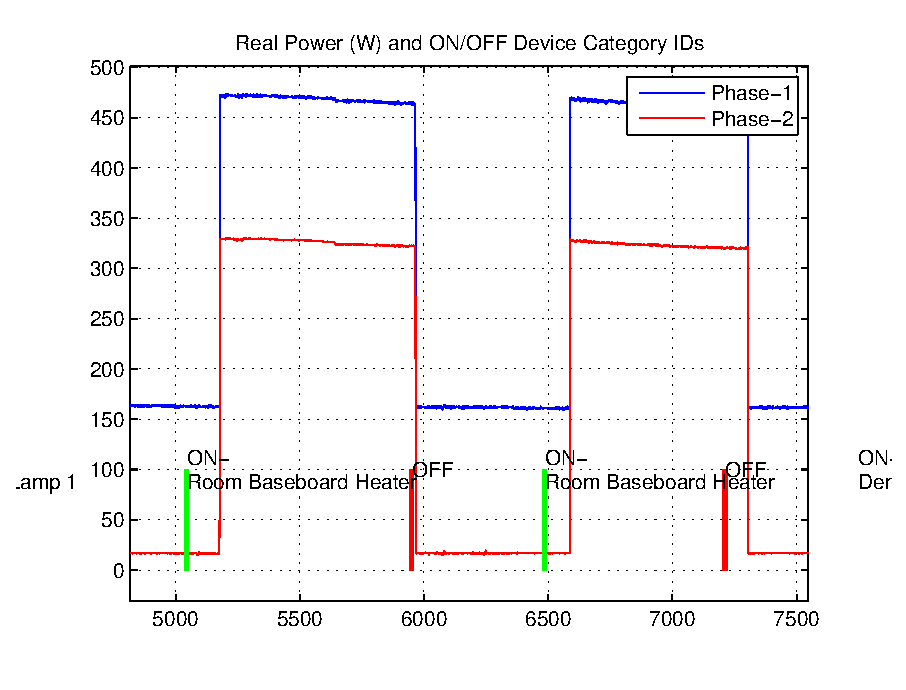
\includegraphics[height=6.5cm]{fig/heater.eps}
\caption{Heater consuming powers from both phases}
\label{fig:heater}
\end{figure}

\subsection{Classification Using DT and k-NN}
Decision trees and k-nearest neighbor classifiers are trained using the real and reactive power consumption features of each home.  The reasons for using these classifiers are: first, both decision tree and k-nearest neighbor can directly classify multi-labeled appliances and second, they are simple and highly interpretable.  The decision tree learning is controlled by reducing the \textit{minsplit} in rpart package provided in R. This is to ensure that the number of leaves exceed the number of labels of the appliances.  For k-nearest neighbor, only k=1 or k=3 can be used since maximum number of 4 observations are available for each appliance.  
\begin{figure}[!ht]
  \centering
  \subfigure[][]{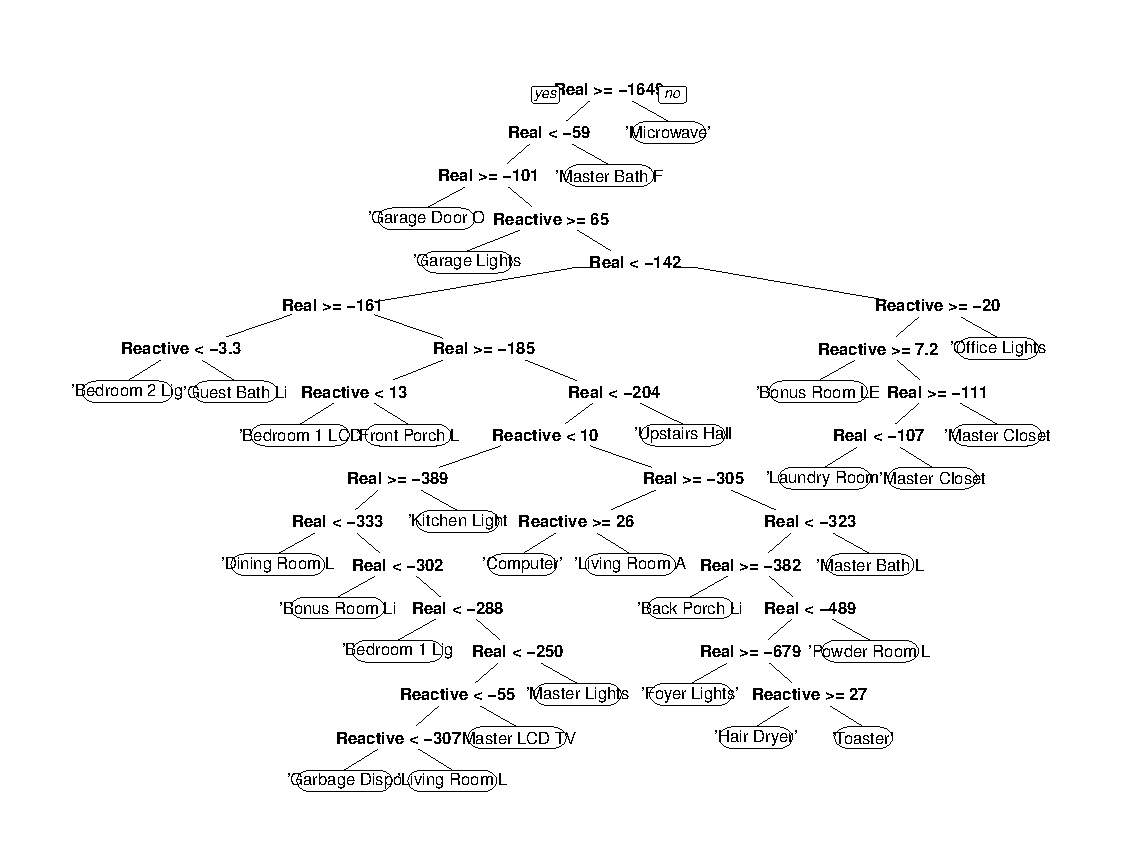
\includegraphics[width=.85\textwidth]{fig/H3_DT.eps}}\quad
  \subfigure[][]{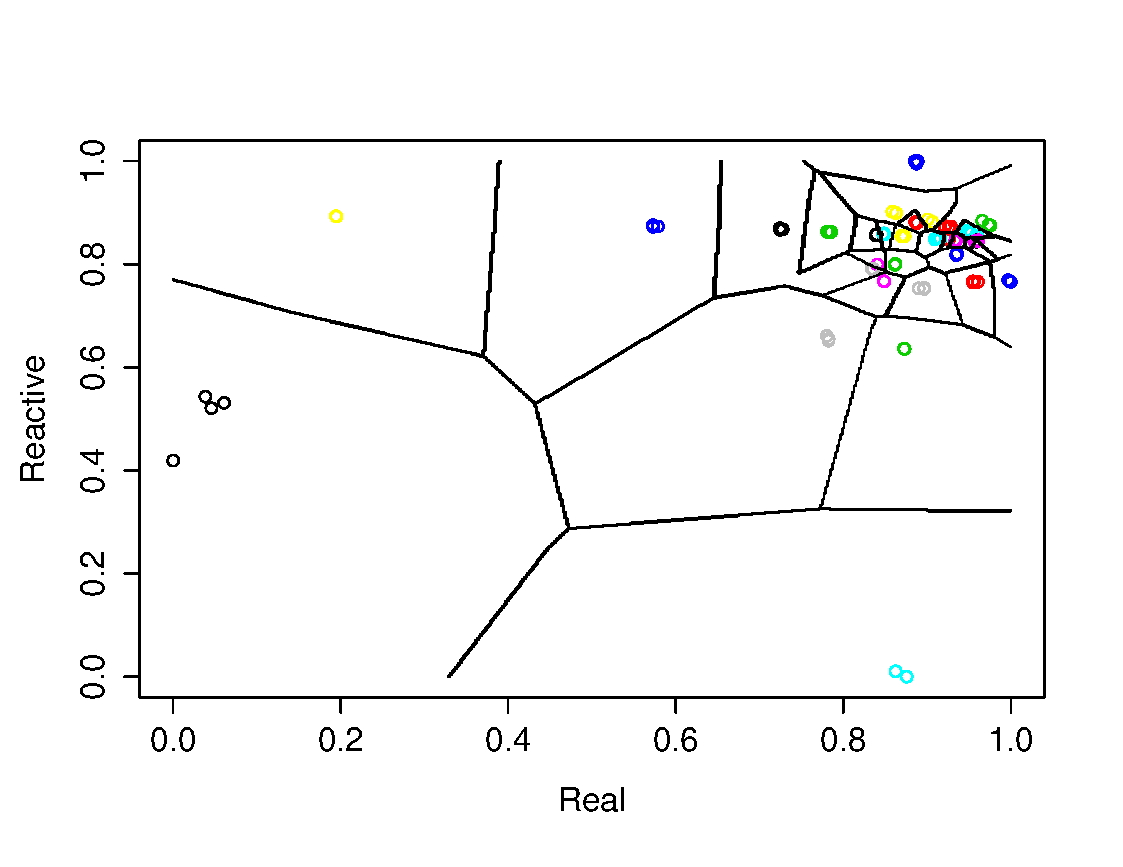
\includegraphics[width=.5\textwidth]{fig/H3_kNN.eps}}\\
  \caption{Classifier induced from Home 3 Training Data (a) decision tree (b) k-NN}
  \label{fig:Classifier}
\end{figure}

\subsection{Leave-one-out Cross-Validation}
Leave-one-out (LOO) cross-validation is performed to the training data.  Even if the data size is large, there are only about four observations for each appliance operating.  Leaving out more than one observation will have considerable impact in performance estimation.  Only the appliances in the white list from Table \ref{tab:LFList} are used in the cross-validation.  The cross-validation results indicate that using real and reactive power consumption alone can classify most of the appliances with high accuracy.
Table \ref{tab:loo} summarizes the classification rate of all the training data. The k-nearest neighbor classifier using k=1 shows the highest classification rate.
\begin{table}[h]
\caption{LOO Cross-Validation Results Using DT and k-NN}
\begin{center}
\begin{tabular}{|p{1.5cm}|p{3.5cm}|p{3.5cm}|p{3.5cm}|}\hline
\textbf{Home} & \textbf{Classification Rate (\%, DT)}& \textbf{Classification Rate (\%, 1-NN)}& \textbf{Classification Rate (\%, 3-NN)}\\
\hline
Home 1 & 89.28571 & 96.42857 & 85.71429\\
\hline
Home 2 & 93.75 & 96.875 & 76.04167\\
\hline
Home 3 & 83.63636 & 98.18182 & 87.27273\\
\hline
Home 4 & 89.65517 & 95.4023 & 90.8046\\
\hline
\end{tabular}
\end{center}
\label{tab:loo}
\end{table}





\section{Appliance Classification Using EMI Data}\label{hfapproach}
Many modern appliances use switched mode power supplies (SMPS). When an appliance is turned on or off, this switching circuit inside the appliance generates an electromagnetic interference pattern. Different appliances generate different patterns. This opens up the possibility of detecting appliance activities and identifying appliances from the measured EMI data. In this section, we explain our methods for event detection, feature extraction, and appliance classification using measured EMI data, which we simply call high frequency (HF) data.

\begin{figure}[H]
\begin{center}
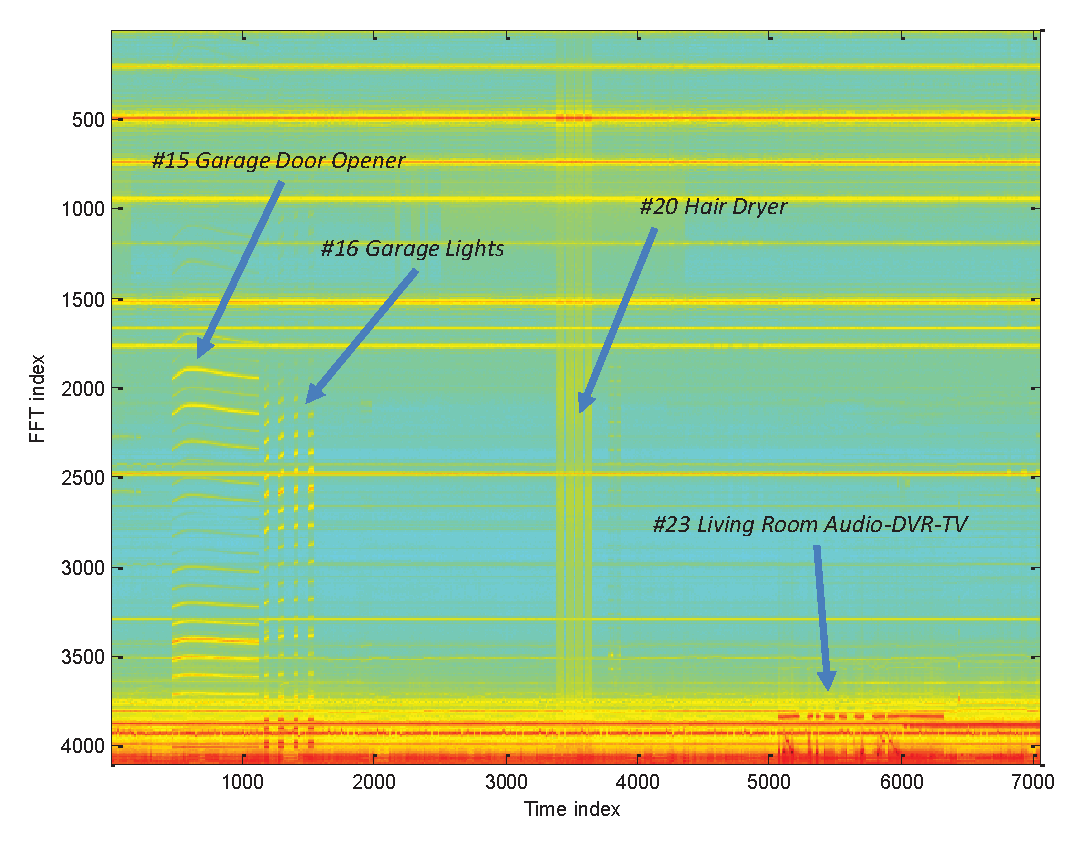
\includegraphics[width=5.0in]{H3_heatmap.eps}
  \caption{Heatmap of appliance EMI pattern for Home 3 training data. Each appliance shows a unique EMI pattern, which is a 4096-point FFT vector, changing over time as appliances are turned on and off.}
  \label{fig:H3_heatmap}
\end{center}
\end{figure}
Figure \ref{fig:H3_heatmap} shows a heatmap of appliance EMI patterns. The data with On/Off time tags is included in the training dataset for Home 3 (H3). We can see that some of the appliances generate very unique patterns, each of which distinguishes itself from the background noise and from the other appliances' patterns. For some types of appliances, the EMI pattern alone is a good separator without help of low frequency (LF) data. Unfortunately, not all the appliances generate strong enough EMI patterns to be used for event detection and appliance classification. Still, HF data analysis is a good complement of the LF data analysis as HF data can separate some of the appliances that are not well separable in LF data.

During our project, the most time consuming part has been defining features such that appliances are well separable and extracting clear-cut features of each appliance from the training data to construct an appliance HF signature database (DB).

\subsection{Event Detection}
Event detection in HF data is performed independently of that in LF data. Let $\mathbf{x}(t)=(x_1(t),x_2(t),...,x_{4096}(t))$ denote the 4096-point FFT vector at (discrete) time instance $t$. Event detection is performed in the following steps:
\begin{itemize}
\item If EMI spectrum fluctuation is large enough, i.e.,
\[\max_{d}[|x_d(t)-x_d(t-1)|]>\mbox{Threshold},\]
Mark the time as $t=T_{change}$.
\item Calculate the difference between two FFT vectors around $T_{change}$,
\[\mathbf{x}_{\mbox{diff}}=\frac{1}{L}\sum_{l=1}^L \mathbf{x}(T_{change}+l)-\frac{1}{L}\sum_{l=1}^L \mathbf{x}(T_{change}-l)\]
where we use $L$-window averaging to smoothe out transient fluctuations and extract steady state difference.
\end{itemize}

\subsection{Feature Extraction}
\begin{figure}
\begin{center}
\includegraphics[width=6.0in]{freq_binning.eps}
  \caption{Frequency binning: Among 4096 FFT dimensions, the lower 2500 frequency bins are taken, and every 100 bins are averaged to become a single bin. As a result, we get a 25-dimension real vector.}
  \label{fig:freq_binning}
\end{center}
\end{figure}

The calculated 4096-dimension difference vector has much more frequency resolution than we need. To reduce dimension, we use frequency binning as described in Figure \ref{fig:freq_binning}. Since we have observed that not many appliances have strong patterns in the upper 1500 frequency bins, we decided to ignore the upper 1596 dimensions and take the lower 2500 frequency bins. After that, we group every 100 bins as a frequency bin, and average out the magnitudes in the same bin. As a result, we have a 25-dimension real vector, which we found to be a good tradeoff between complexity and performance.

We initially tried to perform Gaussian curve fitting on the difference vector and extract the fitted curve parameters as features. However, we have found that most of the appliances have many peaks in their EMI patterns, and also the number of peaks varies much from appliance to appliance, so the Gaussian curve fitting does not give desirable results. After much trial and error, we decided to use the current methods.

From training dataset with On/Off time tags, we extract the HF signature, 25-dimensional vector, from each appliance that generates a strong enough EMI pattern. Using this, we construct the HF signature DB. Note that in the training dataset, most of the appliances appears (turned on and off) 3 or 4 consecutive times, so we extract multiple copies of the same signature that are slightly different due to background noise or interference from other appliances.

\subsection{Appliance Classification}
\begin{figure}
\begin{center}
\includegraphics[width=3.0in]{dist_vs_corr.eps}
  \caption{K-Nearest Neighbor (KNN): Euclidean distance versus correlation.}
  \label{fig:dist_vs_corr}
\end{center}
\end{figure}

For appliance classification, we use two types of K-Nearest Neighbor (KNN) rules:
\begin{itemize}
\item KNN with Euclidean distance \[\min_{j\in\mathcal{A}} \|\mathbf{u}-\mathbf{v}_j\|, \]
\item KNN with correlation \[\min_{j\in\mathcal{A}} \frac{\mathbf{u}^T\mathbf{v}_j}{\|\mathbf{u}\|\|\mathbf{v}_j\|}, \]
\end{itemize}
where $\mathbf{u}$ is the detected HF feature vector, $\mathbf{v}_j$ is the HF signature of appliance $j$, and $\mathcal{A}$ is the set of appliances in the HF signature DB. Figure \ref{fig:dist_vs_corr} shows an example of appliance signature vectors distributed around the detected feature vector in the 25-dimensional vector space. Based on KNN with Euclidean distance rule, 2 nearest neighbors are Garage Lights and Dryer. In contrast, based on KNN with correlation rule, 2 nearest neighbors are Dishwasher and TV since their angles from the detected signature are smaller. We use the mixture of two rules in the following way:
\begin{itemize}
\item First, find the K nearest neighbors based on correlation rule, equivalently, find the signatures within some range of angle from the detected signature. For example, these are dishwasher and TV in Figure \ref{fig:dist_vs_corr}.
\item Second, among those found, choose the one with the minimum Euclidean distance as matching signature. For example, it is the dishwasher in the Figure \ref{fig:dist_vs_corr}.
\end{itemize}


\section{Multi-Classifier Combining}\label{combined}
In the previous section, we saw that neither LF analysis nor HF analysis cover the entire appliance space. Figure \ref{fig:Venn_diagram} shows an example Venn diagram of LF and HF whitelists, which are the lists of appliances well-separable in LF and HF, respectively. As described in Figure \ref{fig:block_diagram}, we use separate classifiers for LF and HF analysis and combine their opinions with appropriate weights. We use the following combining rule:
\begin{itemize}
\item If LF classifier determines that the detected signature belongs to a specific appliance, and the appliance is on the LF whitelist, we give full weight to LF classifier and do not ask HF classifier for its opinion.
\item If LF classifier determines that the detected signature belongs to a specific appliance, but the appliance is on the LF blacklist, the complement set of LF whitelist, we give the weight $1-a$ to LF classifier and the weight $a$ to HF classifier.
\item The weight $a$ is a parameter that depends on the reliability of HF classifier's opinion. For example, if the first and the second nearest neighbors are the same appliance and very close to the detected signature, we give $a=0.9$. In contrast, if they are different appliances or the first appliance is not very close to the detected signature, we give $a=0.5$.
\end{itemize}



\begin{figure}[H]
\begin{center}
\includegraphics[width=4.0in]{Venn_diagram.eps}
  \caption{A Venn diagram showing the appliances that are not well separable in LF data (LF blacklist) but well separable in HF data (HF whitelist).}
  \label{fig:Venn_diagram}
\end{center}
\end{figure}

\begin{figure}[H]
\begin{center}
\includegraphics[width=4.0in]{block_diagram.eps}
  \caption{System block diagram for multi-classifier combiner and the combining rule.}
  \label{fig:block_diagram}
\end{center}
\vskip -15pt
\end{figure}
\section{Results of Approaches}

Each classifier performs reasonably well for the whitelist appliances in the training data.  Performance on the test data is not as accurate due to difficulty in event detection.  However, we did submit our  solutions for the competition at kaggle.com.  Our best score received a mean Hamming Loss of 0.07179, which is the same as the benchmark score.  This benchmark score is for a solution with every appliance off at all timestamps.  Although, our approach was not able to improve on the benchmark, the best solution for a large percentage of teams falls below this.  Our benchmark score places us at approximately 39th out of 165 teams.  This indicates that the classifier should only make an ON prediction for classifications with high confidence to avoid a large penalty. In our approach, this corresponds to setting the threshold of the event detector to be high. 

\section{Key Findings and Lessons Learned}
We have learned from class that having a well processed feature set often results in higher prediction accuracy than applying complex classifiers.  In this project, this turned out to be the event detection and extracting the features from detected events.  The time we spent in extracting the features covered the majority of our time.  Initially, this problem seemed straightforward.  Using LF features alone resulted in more than a 95\% accuracy in cross-validation.  If we were able to detect the events as accurately as in the training data, we expect similar accuracy for the test data.  Unfortunately, the issue lies in the fact that there are no ground truth labels for event occurrence in the test data and therefore we cannot verify the accuracy of event detectors in the test set.  Even when we added the HF features to the LF features, the final evaluation Hamming loss on the test data stayed the same due to the uncertainty in the event occurrence.  Therefore, we suspect that much of the error in the test set classification came from incorrect event detection.  

\section{Conclusion}

From our work on this project, our main conclusion is that the problem of household energy disaggregation can be a well separable classification problem in the feature space that we examined.  However, this is contingent upon accurate event detection, particularly in the presence of simultaneous loads or non-stationary loads, such as dryers and dish washers.  Classification rates in the the training sets were high due to accurate event detection.  Accurate detection was facilitated in part due to availability of tagging information, even considering offsets and mislabels.  However, in the test set we are unable to validate the performance of the event detector resulting in much uncertainty.    

\begin{center}
\textbf{All members contributed (approx) equally to the project. }
\end{center}

\begin{table}[H]
\caption{Appliances well characterized using LF features}
\begin{center}
\begin{tabular}{|p{2cm}|p{9.5cm}|p{3.8cm}|}\hline
\textbf{Home} & \textbf{White List} & \textbf{Black List}\\
\hline
Home 1 & 
BR1 Closet Light, BR1 DVD, BR1 Lights, BR2 Closet Light, BR2 Lights, Coffee Maker, Dining Room Lights, Downstairs Bathroom Fan, Downstairs Bathroom Fan Lights, Downstairs Bathroom Lights, Downstairs Hallway Lights, GR Lights, Garage Lights, Kitchen Lights, Kitchen Under Cabinet Lights, Master BA Heat Lamp, Master BA Lights, Master BR Entry Lights, Master BR Lights, Master BR Walk-in Closet Lights, Outside Over Garage Lights, Over Sink Light, Portable Vacuum, Toaster, Upstairs Hallway Lights
 &
Backyard Light, Balcony Lights, Central Vacuum, Dishwasher, Dryer, GR LCD TV, GR PS4, Garage Door Opener, Outside Front Door Lights, Stairway Lights
\\
\hline
Home 2 & 
Master Bath Fan, Bathroom 1 Lights, Bathroom 2 Lights, Bedroom 1 Lights, Bedroom 2 Lights, Coffee Maker, Computer, Crockpot, Dining Room Lights, Front Hall Lights, Front Room Lights, Garbage Disposal, Hair Dryer, Hallway Lights, Kitchen Lights, Kitchen Table Lights, Laptop Charger, Laundry Room Lights, Living Room Lights, Master Bath Fan, Master Bath Lights, Master Bedroom Lights, Master Closet Lights, Microwave, Office Lights, Outdoor Lights, Refrigerator, Stairway Lights, Straightening Iron, Tea Kettle, Toaster, Vacuum
&  
Dishwasher, Dryer, Phone Charger, Printer, TV/DVR, Washer\\
\hline
Home 3 &  
Back Porch Lights, Bedroom 1 LCD TV, Bedroom 1 Lights, Bedroom 2 Lights, Bonus Room LED TV, Bonus Room Lights, Computer, Dining Room Lights, Foyer Lights, Garage Lights, Garbage Disposal, Guest Bath Lights, Hair Dryer, Kitchen Lights, Laundry Room Lights, Living Room Audio-DVR-TV, Living Room Lights, Front Porch Lights, Master Bath Fan, Master Bath Lights, Master Closet Lights, Master LCD TV/DVR, Master Lights, Microwave, Office Lights, Powder Room Lights, Toaster, Upstairs Hallway Lights
&
Garage Door Opener, Bonus Room Blueray/DVD, Bonus Room Wii, Guest Bath Fan, Master Blueray/DVD, Oven, Dishwasher, Dryer, Washer
\\
\hline
Home 4 &  
Apple Macbook Pro 13, Bedroom Lamp 1, Bedroom Lamps 2, Closet Light, Deck Light, Den Baseboard Heater, Den Overhead Light, Electric Furnace, Forced-air Heater, HP Elitebook Laptop, Hairdryer, Hallway overhead Light, Kettle, Kitchen Counter Lights, Kitchen Lights with Dimmer, LivingRoom overhead halogen, Livingroom Lamp 1, Livingroom Lamp 2, Microwave, Mixer, Oven, PC, PS3, Room Baseboard Heater, Sandwich Maker, Stove, Toaster Oven, Toilet Exhaust, Toilet Halogen, Vaccum
& 
Bose iPhone Dock, Bread Maker, Computer Desk Lamp, Dishwasher, Entry light
\\
\hline
\end{tabular}
\end{center}
\label{tab:LFList}
\end{table}

\begin{table}[H]
\caption{Appliances well characterized using HF features (Home 1 and Home 2)}
\begin{center}
\begin{tabular}{|p{2cm}|p{6.0cm}|p{7.0cm}|}\hline
\textbf{Home} & \textbf{White List} & \textbf{Black List}\\
\hline
Home 1 & 
BR1 Closet Lights,
BR1 Lights,
Backyard Lights,
Balcony Lights,
Central Vacuum,
Dining Room Lights,
Downstairs Bathroom Lights,
Downstairs Hallway Lights,
GR Lights,
GR PS4,
Garage Door Opener,
Garage Lights,
Kitchen Lights,
Kitchen Under Cabinet Lights,
Master BR Lights,
Master BR Walk-in Closet Lights,
Outside Front Door Lights,
Outside Over Garage Lights,
Portable Vacuum,
Power Rm Lights,
Stairway Lights,
Upstairs Hallway Lights,
Washer
&
BR1 DVD, BR2 Closet Light, BR2 Lights, Coffee Maker, Dining Room Lights, Downstairs Bathroom Fan, Downstairs Bathroom Fan Lights, Master BA Heat Lamp, Master BA Lights, Master BR Entry Lights, Over Sink Light, Toaster, Upstairs Hallway Lights, Dishwasher, Dryer, GR LCD TV
\\
\hline
Home 2 & 
Coffee Maker,
Hair Dryer,
Printer
&
Master Bath Fan, Bathroom 1 Lights, Bathroom 2 Lights, Bedroom 1 Lights, Bedroom 2 Lights, omputer, Crockpot, Dining Room Lights, Front Hall Lights, Front Room Lights, Garbage Disposal, Hallway Lights, Kitchen Lights, Kitchen Table Lights, Laptop Charger, Laundry Room Lights, Living Room Lights, Master Bath Fan, Master Bath Lights, Master Bedroom Lights, Master Closet Lights, Microwave, Office Lights, Outdoor Lights, Refrigerator, Stairway Lights, Straightening Iron, Tea Kettle, Toaster, Vacuum,
Dishwasher, Dryer, Phone Charger, TV/DVR, Washer
\\
\hline
\end{tabular}
\end{center}
\label{tab:HFList}
\end{table}

\begin{table}[H]
\caption{Appliances well characterized using HF features (Home 3 and Home 4)}
\begin{center}
\begin{tabular}{|p{2cm}|p{6.0cm}|p{7.0cm}|}\hline
\textbf{Home} & \textbf{White List} & \textbf{Black List}\\
\hline
Home 3 &  
Bedroom 1 LCD TV,
Dishwasher,
Dryer,
Front Porch Lights,
Garage Lights,
Hair Dryer,
Living Room Audio-DVR-TV,
Master LCD TV/DVR,
Office Lights
&
Back Porch Lights, Bedroom 1 Lights, Bedroom 2 Lights, Bonus Room LED TV, Bonus Room Lights, Computer, Dining Room Lights, Foyer Lights, Garbage Disposal, Guest Bath Lights, Kitchen Lights, Laundry Room Lights, Living Room Lights, Master Bath Fan, Master Bath Lights, Master Closet Lights, Master Lights, Microwave, Powder Room Lights, Toaster, Upstairs Hallway Lights,
Garage Door Opener, Bonus Room Blueray/DVD, Bonus Room Wii, Guest Bath Fan, Master Blueray/DVD, Oven, Washer
\\
\hline
Home 4 &
'Stove' 'Kitchen Lights with Dimmer' 'Vaccum' 'Hairdryer' 'Den Baseboard Heater'
'Forced-air Heater' 'PS3' 'Livingroom Lamp 1' 'Livingroom Lamp 2' 'Den Overhead Light' 'Entry light'
'Hallway overhead Light' 'Closet Light'
'HP Elitebook Laptop' 'Apple Macbook Pro 15'
&
'Microwave'
'Toaster Oven'
'Bread Maker'
'Kettle'
'Mixer'
'Sandwich Maker'
'Kitchen Counter Lights'
'Oven'
'Dishwasher'
'Bedroom Lamp 1'
'Bedroom Lamp 2'
'Room Baseboard Heater'
'Electric Furnace'
'Electric Furnace'
'Bose iPhone Dock'
'PC'
'Computer Desk Lamp'
'LivingRoom overhead halogen'
'Deck Light'
'Toilet Halogen'
'Toilet Exhaust'
'Apple Macbook Pro 13'
\\
\hline
\end{tabular}
\end{center}
\label{tab:HFList}
\end{table}

\newpage
\bibliography{Bib}
\bibliographystyle{ieeetr}


\end{document}
